\subsection{Visual representation}
\label{sec:seg_colors}
For visually representing segmentation, we make a color map over the images, following
the cityscapes color palette \cite{cordts_cityscapes}. See figure \ref{fig:segmentation_colors}
for the exact palette and class list, and figure \ref{fig:cs_sample}

\begin{figure}[ht]
	\begin{center}
	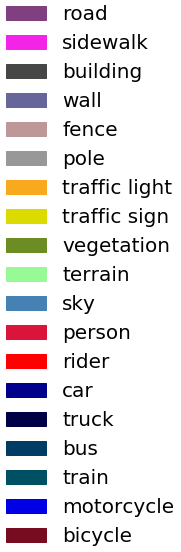
\includegraphics[width=0.2\textwidth]{./figures/seg_colors.png}
	\caption[Segmentation color palette]{
        Segmentation color palette.
        }
	\label{fig:segmentation_colors}
	\end{center}
\end{figure}

\begin{figure}[ht]
	\begin{center}
	\includegraphics[width=1\textwidth]{./figures/cityscapes_sample.png}
	\caption[CityScapes sample]{
        CityScapes sample.
        }
	\label{fig:cs_sample}
	\end{center}
\end{figure}